\chapter{METHODOLOGY}
\label{ch:system}
\begin{figure}[htbp]
\centering
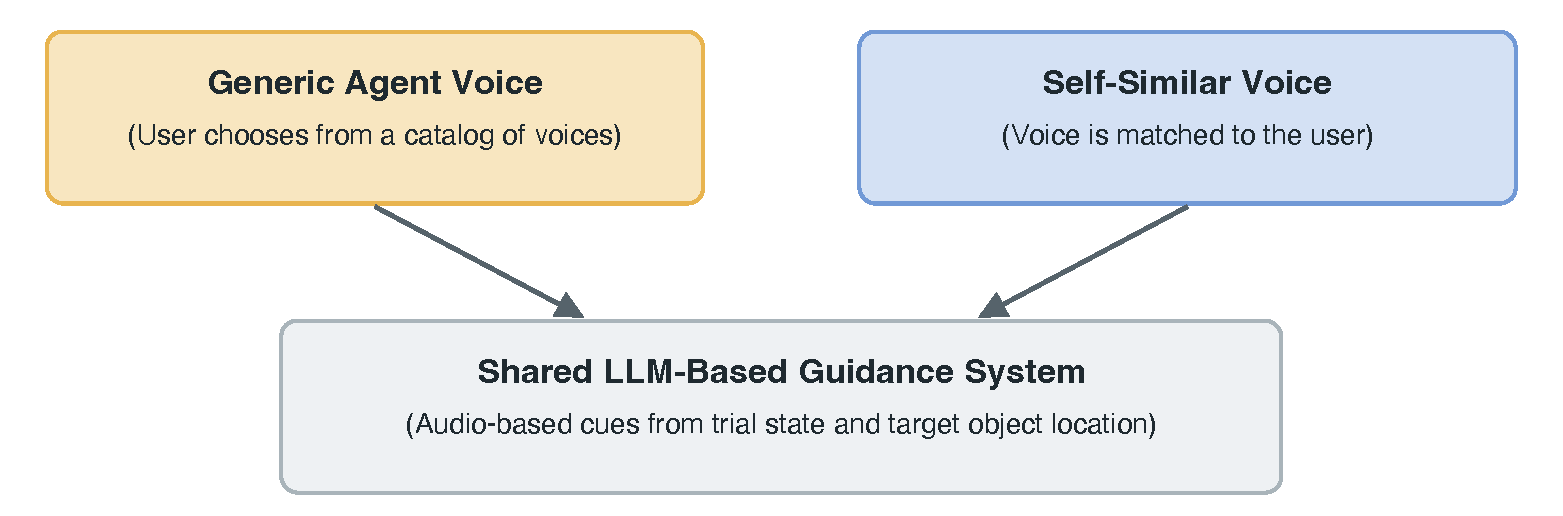
\includegraphics[width=\linewidth,alt={Two voice conditions, a generic agent voice the user chooses from a catalog and a self-similar voice matched to the user, both feed one shared LLM-based guidance system that produces audio cues from the trial state and the target object's location.}]{figures/system-setup.pdf}
\caption[System setup]{System setup. Guidance is delivered in one of two voices: a generic agent voice that the participant chooses from a catalog, or a self-similar voice matched to the participant. Both voices are driven by the same guidance system, which issues audio cues from the trial state and the target object's location.}
\label{fig:system-setup}
\end{figure}
This chapter outlines the application development, experimental design, and data collection methods used in Follow My Voice to evaluate how the voice delivering spoken guidance, either a self-similar voice or a generic agent voice chosen by the participant, impacts object search performance, workload, and engagement. The guidance voice is the independent variable, while the search task and the gaze-contingent agent guidance system remain the same across conditions. The application is created in Unity 6 (6000.3.10f1) for the HTC VIVE Focus Vision headset (2448 $\times$ 2448 resolution per eye, 90-Hz refresh rate, up to 120$^\circ$ field of view, integrated eye tracking) using the Unity OpenXR Plugin and the HTC VIVE OpenXR integration~\cite{htc2026focusvision}.

In the experiment, participants complete one practice trial and then two counterbalanced blocks of 40 trials, with each block representing a different voice condition. Each trial begins in the same way: participants search for a specific target among colored geometric objects on eight surrounding walls while the agent guides them with spoken directions. Participants do not know what the object is ahead of time. The source code is available at \url{https://github.com/PedroPovedaQ/Gaze-Contingency-Project}. Performance and eye-tracking data are collected through the headset application, and perceived workload, voice preference, and task engagement are captured through questionnaires.

\section{Application Design}
\label{sec:application-design}
\subsection{Apparatus and Search Scene}
The application is developed in Unity 6 (6000.3.10f1) using the Unity OpenXR Plugin (1.16.1), HTC VIVE OpenXR integration (2.5.1), and Unity XR Interaction Toolkit (3.3.1). It is deployed as a standalone Android ARM64 application on the HTC VIVE Focus Vision head-mounted display, with rendering performed locally on the headset using the Universal Render Pipeline (17.3.0). The study uses the headset's virtual-reality configuration, in which the headset supplies head-pose and eye-gaze tracking and the tracked right-hand controller supplies pointing and trigger input. Network access supports voice preparation and the connection to the lab computer that runs the decision model. It is not used to stream rendered frames from a host computer. HTC specifies 2448 $\times$ 2448 pixels per eye, a 90-Hz standalone display refresh rate, and a field of view of up to 120 degrees~\cite{htc2026focusvision}.

\begin{figure}[htbp]
\centering
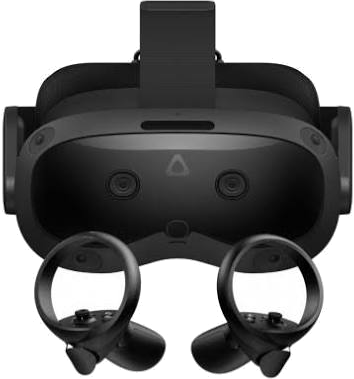
\includegraphics[width=0.42\linewidth,alt={The HTC VIVE Focus Vision head-mounted display, seen from the front, with its two six-degree-of-freedom handheld controllers below it.}]{figures/htc-vive-focus-vision.png}
\caption[HTC VIVE Focus Vision HMD and controllers]{HTC VIVE Focus Vision HMD and controllers. Image: HTC~\cite{htc2026focusvision}.}
\label{fig:htc-vive-focus-vision}
\end{figure}

The search task takes place in a neutral virtual room (Figure~\ref{fig:recorded-search-scene}). The development configuration contains 168 objects, or 21 per plane, at a default plane radius of 1.5~m from the seated origin. These colored geometric objects hover in space and represent the target and its distractors. Figure~\ref{fig:scene} shows the layout from above. The objects are represented in six shapes---sphere, cube, pyramid, cylinder, capsule, and star---in red, blue, yellow, and green. Objects vary in height and horizontal position within their assigned plane, so search requires both coarse orientation toward a plane and finer search within it once the user's gaze approaches the vicinity of the object. The gaze-contingent agent knows the target identity and the user's gaze data but withholds the target's identity from the user; participants must rely on the agent's auditory guidance to locate the target. Participants select the object by pointing the right-controller ray toward it and pressing the trigger.

\paragraph{Project Setup.} Each wall is approximately 2.20~m high. Seat height is adjusted so that participants are better aligned with the readiness cross. Per-trial layouts are procedurally generated from a designated theta, the horizontal angle between the trial's starting direction and the target object (Section~\ref{sec:theta-measures}).

\begin{figure}[htbp]\centering
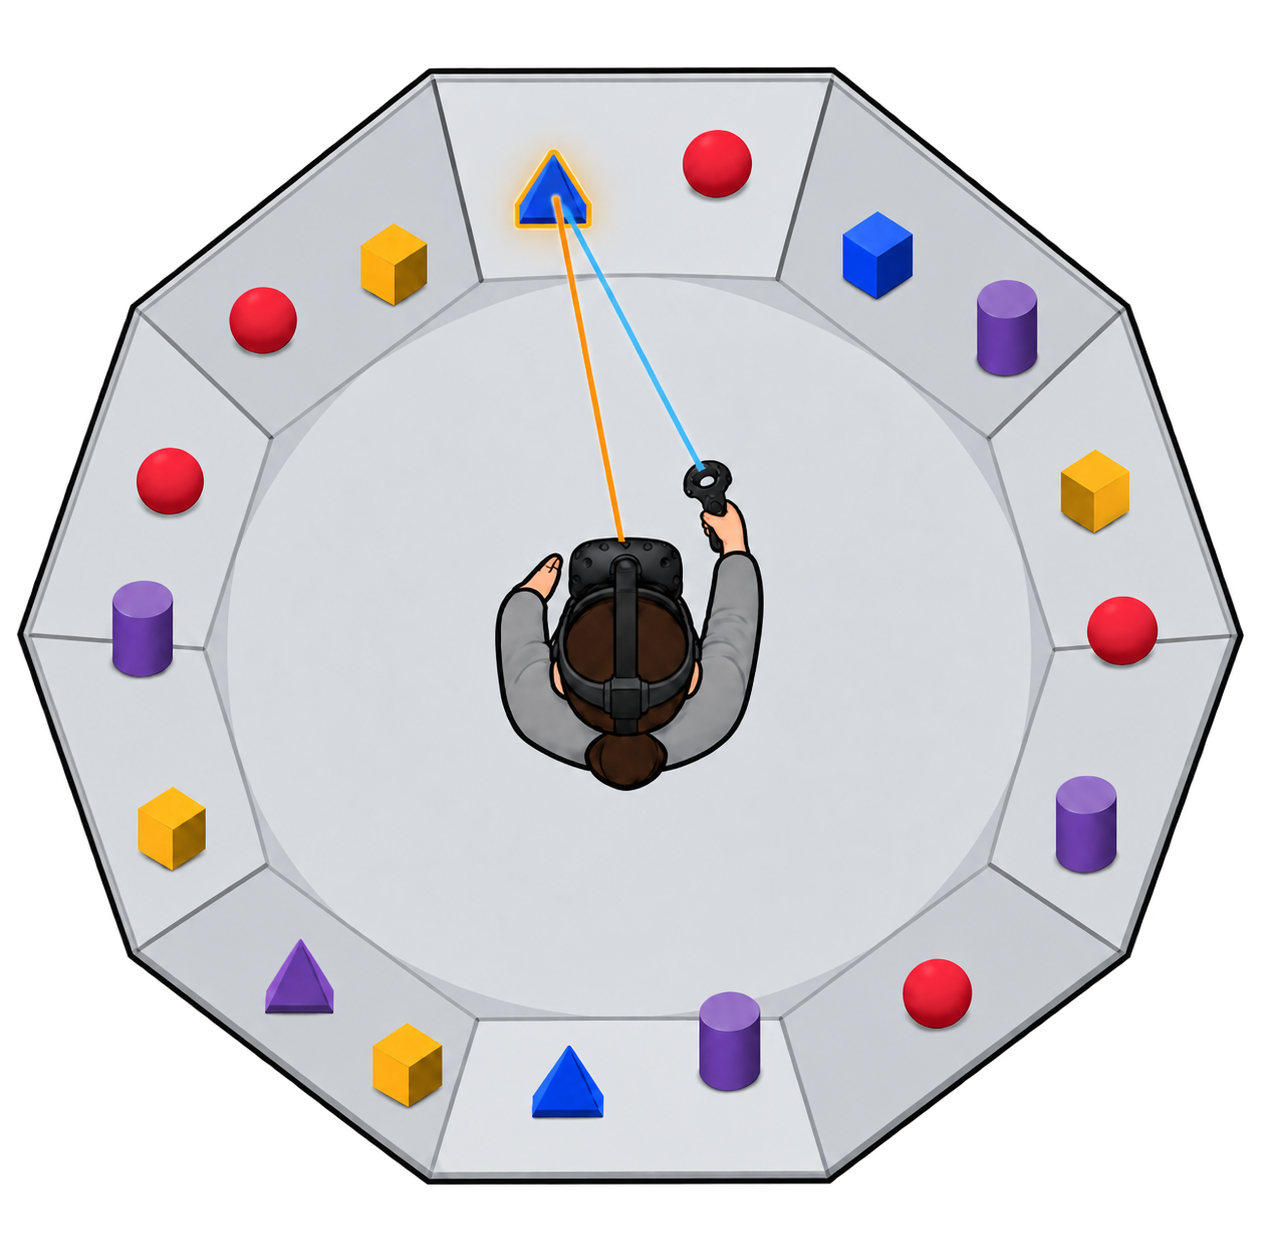
\includegraphics[width=0.70\linewidth,alt={Overhead scene illustration showing a seated headset wearer, surrounding vertical object panels, and gaze and controller rays.}]{figures/image.png}
\caption[Search-scene illustration]{Top-down view of the search scene. The seated participant is surrounded by wall panels holding colored geometric objects. The gaze ray (orange) and controller ray (blue) converge on the highlighted target, representing the state in which the participant is ready to select with the trigger.}
\label{fig:scene}
\end{figure}

Figure~\ref{fig:recorded-search-scene} complements the schematic with a reconstruction from an actual headset development recording.

\begin{figure}[p]\centering
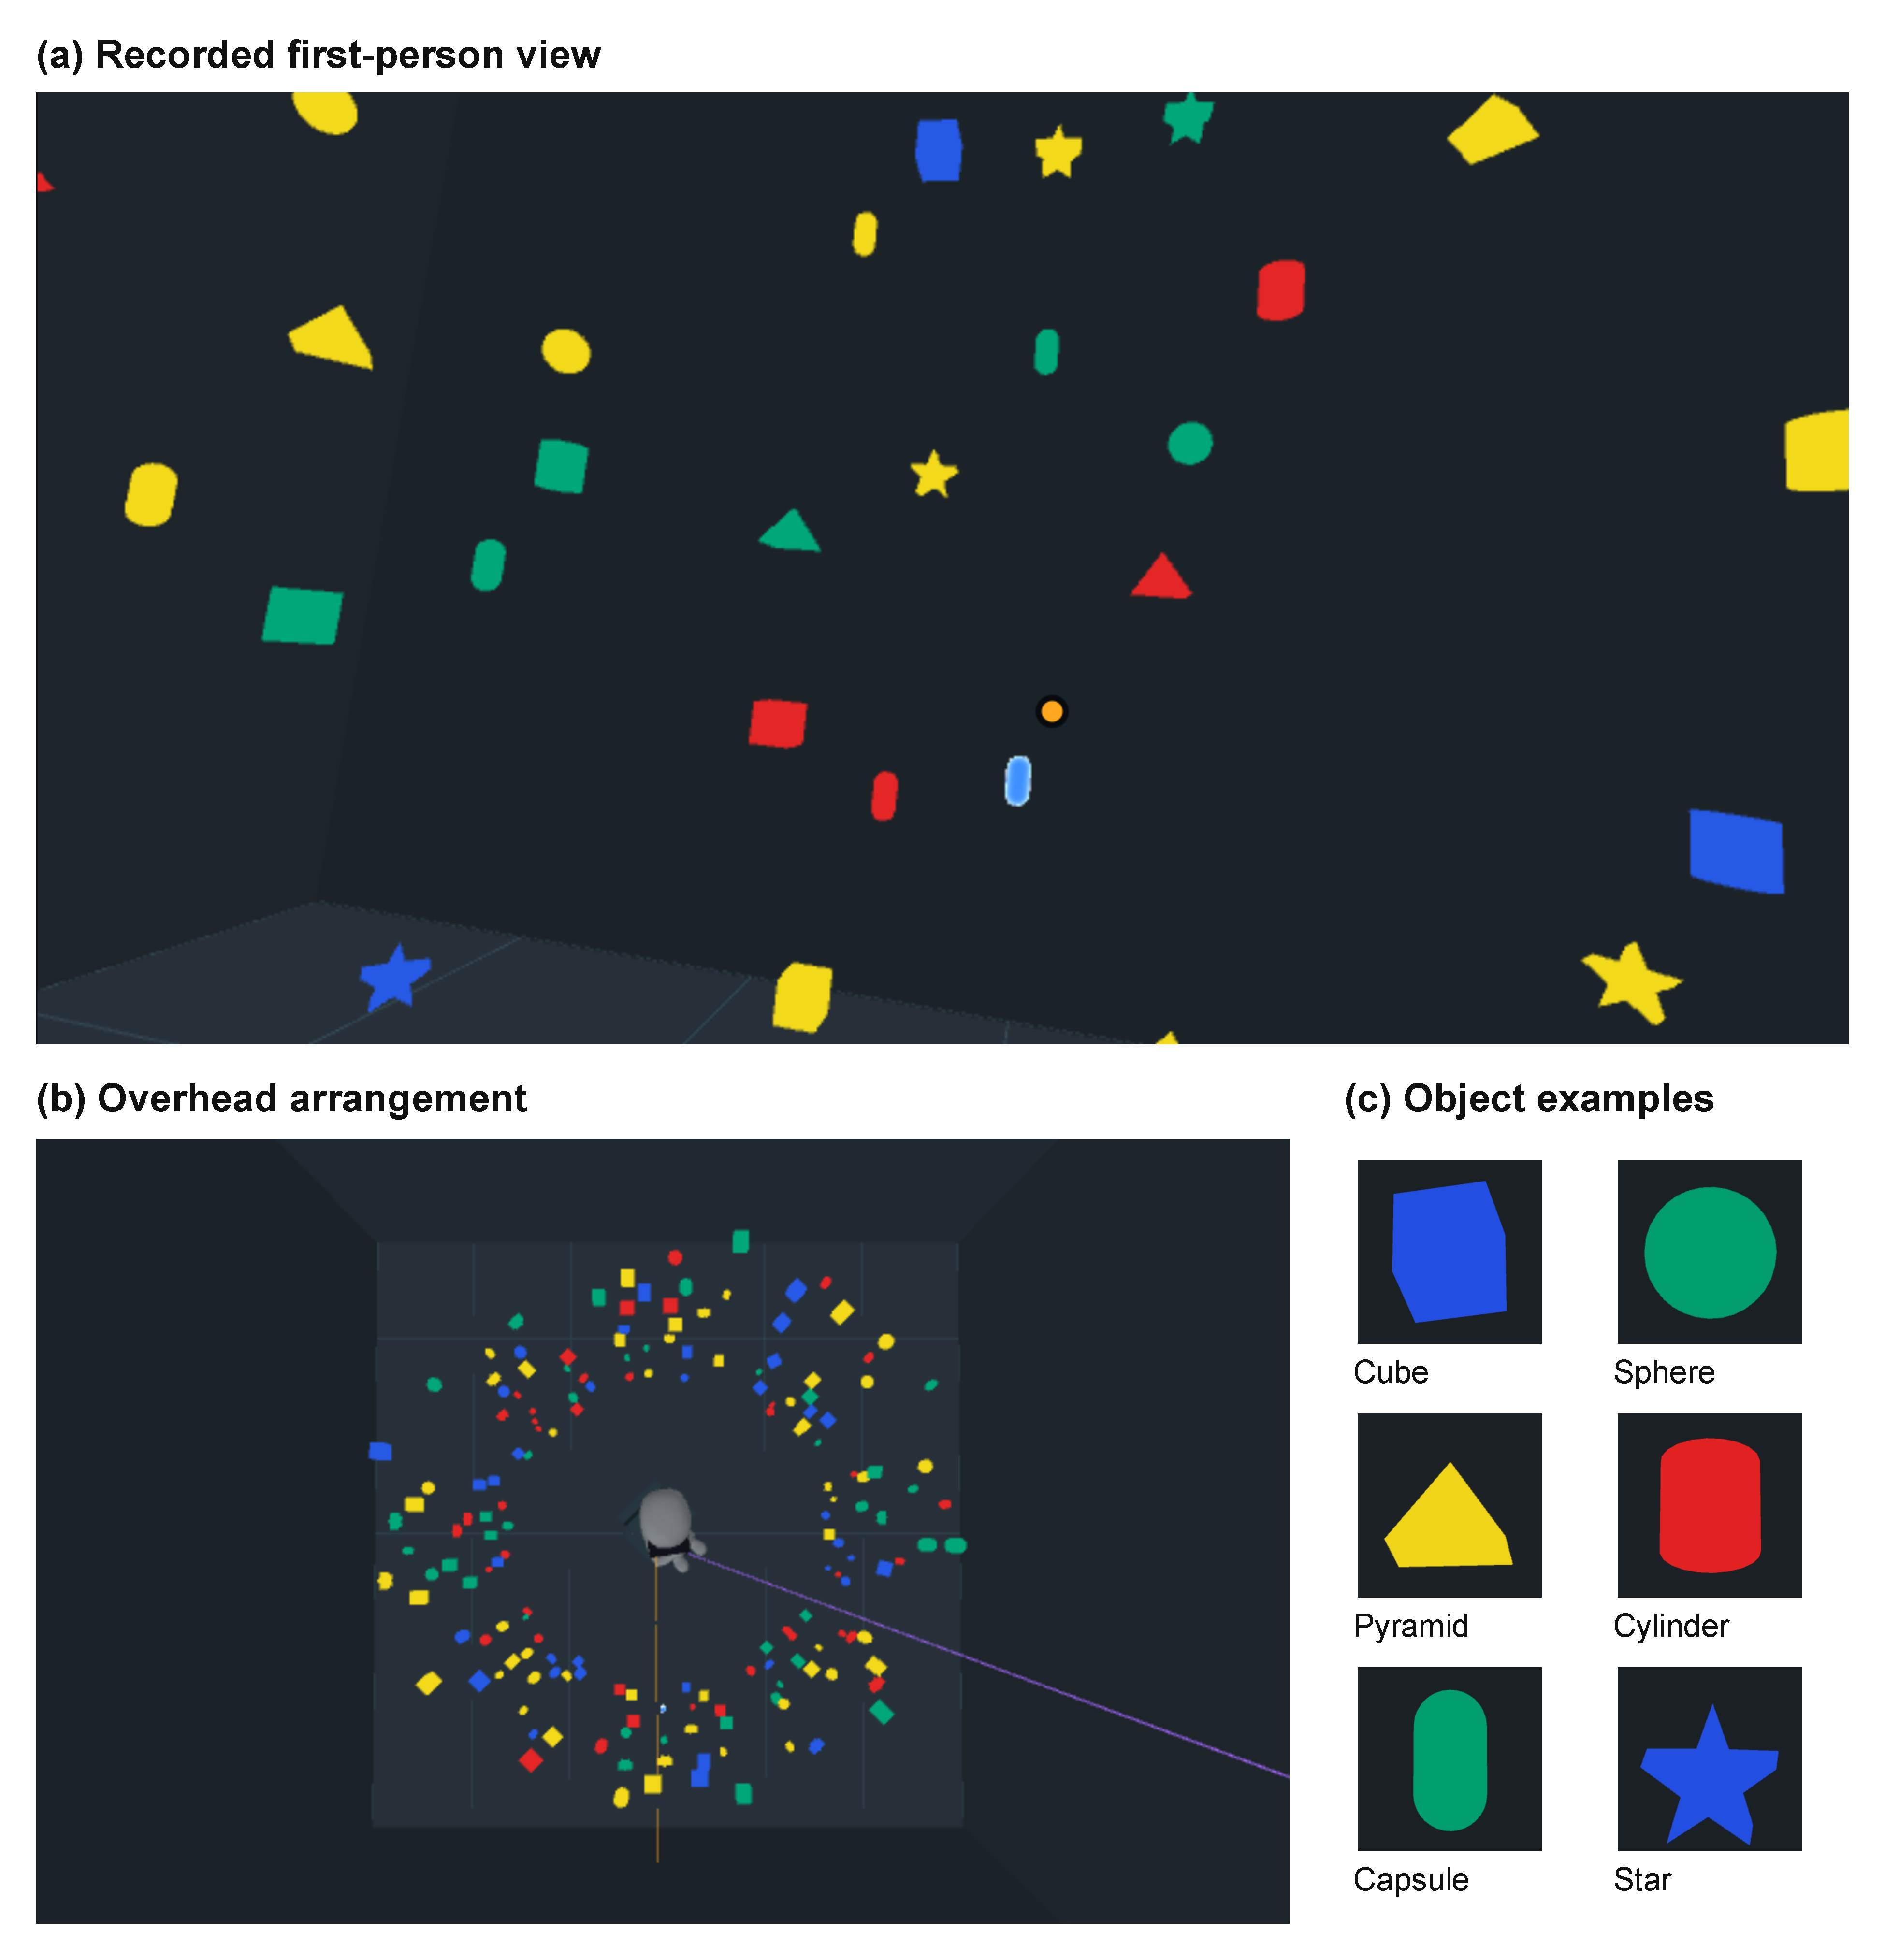
\includegraphics[width=0.92\linewidth,alt={Three-panel reconstruction of the search environment: the recorded first-person view of colored objects on vertical planes; an overhead view of eight surrounding planes and the central wearer avatar; and zoomed cube, sphere, pyramid, cylinder, capsule and star examples.}]{figures/recorded-search-scene.pdf}
\caption[Search environment and object examples]{(a) First-person view of colored objects on surrounding vertical planes. (b) Overhead view of the eight-plane arrangement. (c) Enlarged examples of the six shape types at independent scales. Images are reconstructed from a headset development session recorded before the wall-height reduction and show the earlier wall dimensions; they are development material, not participant-study results.}
\label{fig:recorded-search-scene}
\end{figure}

\subsection{Voices}
Voice cloning, which replicates a speaker's voice from a short reference recording, has become practical with recent instant-cloning methods~\cite{qin2023openvoice}. In this study, all voice audio is pre-synthesized with the commercial ElevenLabs service, which supplies both the neutral voice and the self-similar voice. To support the self-similar condition, the participant's spoken answers during the audio intake provide the samples for cloning, so no separate recording step is needed; a standard reading passage is retained as a fallback when the intake does not yield enough usable speech (Appendix~\ref{app:instruments}). The intake uses its own generic voice so that neither study voice is heard before the practice trial. Both conditions share the semantic phrase library, guidance policy, and playback routing, so voice is the intended manipulation. Because guidance responds to behavior, however, the wording and number of hints can differ between blocks, and the synthesized clips can differ acoustically. The preparation pipeline automatically checks wording and library readiness, but these checks do not assess perceptual equivalence. Pilot sessions will therefore verify per-voice intelligibility, loudness, and acoustic comparability. No pitch or spatial effects are applied to the self-similar voice. The system logs the provider, model, voice ID, library version, and synthesis settings.

The Trial Review application aligns gaze and controller state, guidance transitions, agent decisions, and playback events with trial geometry on a common timeline. Trial-level aggregates are stored separately from the raw gaze, motion, and event streams. The effective gaze sampling rate will be determined from distinct source timestamps on the study headset build rather than from the nominal specification or the application polling rate. The analysis will report ray intersections as gaze hits, which approximate, but are not equivalent to, fixations identified by a validated event classifier~\cite{salvucci2000fixations}.

\subsection{Gaze-Contingent Guidance}
Prior guidance systems combine initial orientation with finer guidance toward the target~\cite{kwok2022twostep,tanaka2026coarse}. Spoken directions in Follow My Voice follow a similar progression. The system updates them from evidence of the participant's progress, so that instructions can shift from orientation toward a wall to refinement around an object. The same sensing and state logic serves both voice conditions.

The system continuously collects eye-gaze origin, direction, and validity; head pose; right-controller pose; and ray-object intersections. A local state machine combines these observations with the target geometry to track the participant's progress through the search: turning toward the target wall, refining within the wall, acquiring the target with gaze, pointing with the controller, and becoming ready to select. Additional states cover suspended or paused operation. Each state transition is logged with its cause.

The state machine issues new gaze-dependent guidance only when gaze data are valid and recent. Gaze ray hits, gaze-vicinity candidates, and controller hits are treated as separate observations; when gaze-vicinity regions overlap, the closest object is chosen as the vicinity candidate. A controller ray hit on the target immediately suppresses contradictory directional cues. The spoken pointing acknowledgment, by contrast, requires a one-second controller hold with valid nearby gaze and plays only when the speech scheduler permits it. Gaze confirmation, controller confirmation, and trigger selection are recorded as distinct events.

\subsubsection{From Gaze to Spoken Direction}
\label{sec:guidance-geometry}
The direction in each cue is computed geometrically by the application before the decision model is consulted, so the model never has to infer which way the target lies. Each valid gaze sample supplies an eye origin $\mathbf{o}$ and a gaze direction $\mathbf{g}$, and the target's position $\mathbf{p}$ is known from the layout. Both $\mathbf{g}$ and the target vector $\mathbf{d}=\mathbf{p}-\mathbf{o}$ are expressed relative to the seated forward direction, so the computation does not depend on how the room is oriented. A sample whose direction lies within about $12^\circ$ of straight up or down is treated as unusable rather than as a departure from the wall, because left and right are undefined there.

\paragraph{Wall membership.} The eight walls form a ring at $45^\circ$ intervals around the chair. The gaze ray is transformed into the target wall's frame and tested against that wall's horizontal sector. Height is ignored in this test, so scanning up and down the correct wall is not counted as leaving it.

\paragraph{Angular error.} The horizontal error $\psi$ is the signed angle about the world up axis between the horizontal projections of $\mathbf{g}$ and $\mathbf{d}$; it is positive when the target lies to the participant's right. The vertical error is the difference in elevation,
\begin{equation}
\phi=\operatorname{elev}(\mathbf{d})-\operatorname{elev}(\mathbf{g}),\qquad
\operatorname{elev}(\mathbf{v})=\operatorname{atan2}\!\left(v_y,\sqrt{v_x^2+v_z^2}\right)\frac{180}{\pi},
\end{equation}
which is positive when the target is higher than the point of regard.

\paragraph{Turning toward the wall.} Outside the target wall, the sign of $\psi$ selects ``left'' or ``right.'' When the target is nearly behind the participant ($|\psi|\geq150^\circ$), the first chosen direction is retained, so small head movements across the rear seam cannot reverse an instruction already given, and the remaining turn is measured along that route. Progress cues are earned in $45^\circ$ steps, one wall at a time: crossing the same step again after turning back does not produce another ``keep going.''

\paragraph{Refinement within the wall.} Inside the target wall, $\phi$ and $\psi$ are converted to one of nine directions: up, down, left, right, the four diagonals, or aligned. A vertical component is added when $|\phi|$ exceeds $3^\circ$, and a horizontal component when $|\psi|$ exceeds $5^\circ$. Once a component is being spoken, it persists until the error falls below $1.5^\circ$ vertically or $3^\circ$ horizontally, and an aligned state persists until the error exceeds $4.5^\circ$ vertically or $7^\circ$ horizontally. These separate entry and exit thresholds prevent small eye movements from flipping the instruction back and forth. They are development settings rather than values drawn from prior work. Within the wall, the gaze ray must also intersect the wall plane so that its vertical position can be measured; otherwise no new direction is issued.

\paragraph{Consistency with the visible highlight.} The object nearest the gaze ray on the target wall receives a visible highlight. If a vertical instruction would contradict that highlight's position relative to the target, for example ``down'' when the target is above the highlighted object, the vertical component is dropped and only the horizontal component is spoken. The system never substitutes the opposite vertical direction.

\paragraph{Target acquisition.} New directional guidance stops once gaze has remained within the target's vicinity ring for at least 100~ms or the controller ray is on the target (Section~\ref{ch:measurement}). The phrases offered to the decision model are limited to those whose direction matches the computed one, and each selected cue is checked against a fresh evaluation of this geometry before playback (Section~\ref{sec:playback-control}).

\subsection{Decision Model}
\label{sec:decision-model}
Follow My Voice uses a small, fine-tuned language model to decide when and how the agent speaks. The model is based on MiniLM~\cite{wang2020minilm}, a compact transformer distilled from a larger language model, in its six-layer \texttt{all-MiniLM-L6-v2} sentence-encoder form~\cite{reimers2019sbert}, with about 22 million parameters. Unlike a large language model, it does not generate free-form text. It is fine-tuned as a classifier that chooses among a small set of guidance strategies, and a second fine-tuned copy ranks the prepared phrases that carry out the chosen strategy. Both voice conditions use the same model and the same phrase library.

\subsubsection{From a Cloud Model to a Local Model}
\label{sec:cloud-to-local}
Guidance decisions were initially made by Jev, a cloud-hosted large language model. Each decision therefore required a request to a remote service, and the resulting latency proved too high for guidance that must keep pace with the participant's head and eye movements. In the development sessions of October 19--20, 2026, for example, one gaze confirmation reached playback 2.19~s after the first qualified request, following repeated requests to the cloud model (Section~\ref{sec:development-results}). The cloud model was therefore replaced with the small local model described in this section, which answered roughly five to six times faster in comparable requests (Section~\ref{sec:small-local-model}). The change did not alter the application's geometry, phrase library, or playback checks. The local model is not a compressed copy of Jev: it was fine-tuned from the pretrained MiniLM checkpoint on synthetic states labeled by an authored reference policy, and Jev's responses were not used as training labels (Section~\ref{sec:model-training}).

\subsubsection{Choice of Base Model}
The base model was chosen for three properties of the task. First, guidance phrases are short spoken sentences, and many differ only in emphasis or degree, such as ``Turn right,'' ``Keep turning right,'' and ``A little more right.'' Sentence-BERT models are trained so that sentences with similar meanings receive similar representations~\cite{reimers2019sbert}, so the starting checkpoint already distinguishes and relates such variants. This prior knowledge allows a moderate amount of synthetic training data to suffice for both the strategy choice and the phrase ranking. Second, the six-layer model is small enough to answer within the time scale of head and eye movement on the lab computer's processor (Section~\ref{sec:small-local-model}). Third, an encoder that classifies and ranks can return only options it was offered. Every phrase is synthesized in advance in both voices, including the participant's clone, and cached on the headset, so a phrase the model selects always has recorded audio in both conditions. A generative model could compose a sentence for which neither voice has a recording, and the two conditions could then diverge in wording. The checkpoint is released under the Apache-2.0 license and pinned to a fixed revision, so the starting weights can be reproduced. Its pretraining on general English text carries no knowledge of the task geometry, which is one reason geometric rules and gating remain outside the model (Section~\ref{sec:overrides}).

\subsubsection{State Sent to the Model}
At each decision point, Unity assembles a structured state of the search. It records whether gaze evidence is valid and recent, whether the participant is inside the target wall, and whether target gaze or controller pointing qualifies. It adds the horizontal and vertical error to the target and its distance band, how that error has changed over the last few seconds (trend, net reduction, and gaps in tracking), the last cue and how the participant responded to it, the number of cues and wrong selections so far, the outcomes of previous trials, the time since speech ended, and the strategies currently allowed. The model receives this state as a compact text description of at most 384 tokens.

\subsubsection{How the Model Decides}
The strategy head chooses one of seven options: observe for one second (stay silent and reassess), brief or explicit orientation toward the target wall, brief or explicit refinement within the wall, correction, or encouragement. Unity offers only the strategies that are valid in the current situation, and the model can choose only among them. When the chosen strategy is to speak, the phrase ranker scores the prepared phrases offered for that strategy, taking into account how often and how recently each phrase has played, and the highest-scoring phrase is scheduled. The model's scores are used only to choose among the offered options; they are not calibrated probabilities.

\subsubsection{Why a Small Local Model}
\label{sec:small-local-model}
Guidance has to keep pace with head and eye movements that change within a fraction of a second, and a cue that arrives late can send the participant somewhere they have already looked. The model therefore runs on the lab computer beside the headset and answers over a local connection. In development measurements on that computer, a complete two-stage decision (strategy and phrase) took about 84--87~ms, and a direct model call about 12--18~ms. For the first phrase on reaching the target wall, the local model responded in 171~ms, whereas the cloud large language model previously used for these decisions, Jev, responded in 820~ms in a single comparable request; an earlier local version showed a median of 30~ms against 182~ms for the cloud model. These timings were taken on the desktop and do not include headset networking or the onset of audible speech. Running locally also keeps the participant's behavioral state on the lab computer, and because the model can only select among prepared phrases, it cannot produce unexpected wording.

\subsubsection{Deterministic Overrides}
\label{sec:overrides}
Guidance is otherwise driven entirely by the model; fixed rules take precedence only in a few specific situations. No decision is requested when gaze is invalid, when the participant is already looking at or pointing at the target, when the guidance state is not a search state, or when audio is not ready, and a server-side gate forces silence under the same conditions. On the first arrival at the target wall in each trial, the strategy is fixed to an explicit refinement and the model chooses only among four area phrases. When the participant reverses direction, an obsolete cue is faded out without replacement. A reminder plays only at the 25-second deadline when the participant is already on the target, and trial openings, target confirmations, and success feedback come from prepared local phrases. Only one request may be pending, requests are at least 0.75~s apart, and any decision older than 3.25~s or no longer matching the participant, trial, voice, or policy version is discarded. If a request fails, the agent stays silent and retries rather than falling back to another provider.

\subsubsection{Short-Term Memory}
The state includes a short-term memory of the participant's behavior. A spatial history samples the error to the target every 0.5~s over the last 12~s and is cleared when tracking is lost for more than 1.25~s. A cue history keeps the last eight cues in the trial and the participant's response to each, measured as the change in error over the following 3~s. A phrase history records how often and how recently each phrase has played, and summaries of the previous six trials carry information across trials. Trial-level memory resets at each new trial and participant-level memory at each new participant. A separate speech memory of the last four speech events within 15~s supports the playback checks described below.

\subsubsection{Training}
\label{sec:model-training}
The model was trained on synthetic decision states generated to cover the situations guidance must handle: stalled, receding, oscillating, steady, and mixed search trajectories, departures from the target, different silences and numbers of prior cues, and failures of the gating conditions. Each state was labeled by an authored reference policy, so that the model learns to reproduce that policy quickly from the compact state. Recorded headset sessions were not used as training examples; instead, real development recordings served as regression tests and shaped successive rounds of synthetic data. The current version was fine-tuned from earlier versions with AdamW for six epochs on 2,240 training states balanced across the seven strategies, with 448 validation and 448 test states generated with different sampling cadences and combined gate failures. It agreed with the reference policy on 94.6\% of test states (95.1\% after the deterministic gates), and the phrase ranker agreed with its reference on 95\% of test cases and avoided repeating a phrase in all 88 opportunities to do so. These figures measure agreement with the authored policy, not usefulness to participants, which the user study will assess.

\subsection{Playback Control}
\label{sec:playback-control}
Because decisions arrive asynchronously, the participant's state may change before a decision returns. A local speech scheduler therefore revalidates each decision against the current state, evidence, pacing, and object intersections before playback, and discards decisions that are stale or conflict with the current situation. Qualified gaze and controller acknowledgments, together with eligible turn-progress milestones, can be handled locally and played from prepared phrases without waiting for a new model decision. These local cues remain subject to the same checks. When a qualified target acknowledgment would replace misleading search speech, a local fast path avoids waiting for interruption advice. This path protects the first 0.35 seconds and final 0.5 seconds of the current phrase, retains a 2.5-second interruption cooldown, and fades the audio over 150 ms. The fast path keeps the separate gaze and controller hold requirements, and fresh evidence is checked before the fade, after it, and at playback. Setup, completion feedback, and existing acknowledgments are protected from interruption. Each completed or interrupted utterance updates both the memory and the event log. Model latency, deferral, cancellation, fallback, and playback onset are logged separately to support delay attribution. When a trace lacks the required events, the source of a delay is recorded as unknown rather than inferred from the spoken phrase alone.

\begin{figure}[htbp]\centering
\IfFileExists{figures/voice-guidance-memory-architecture.pdf}{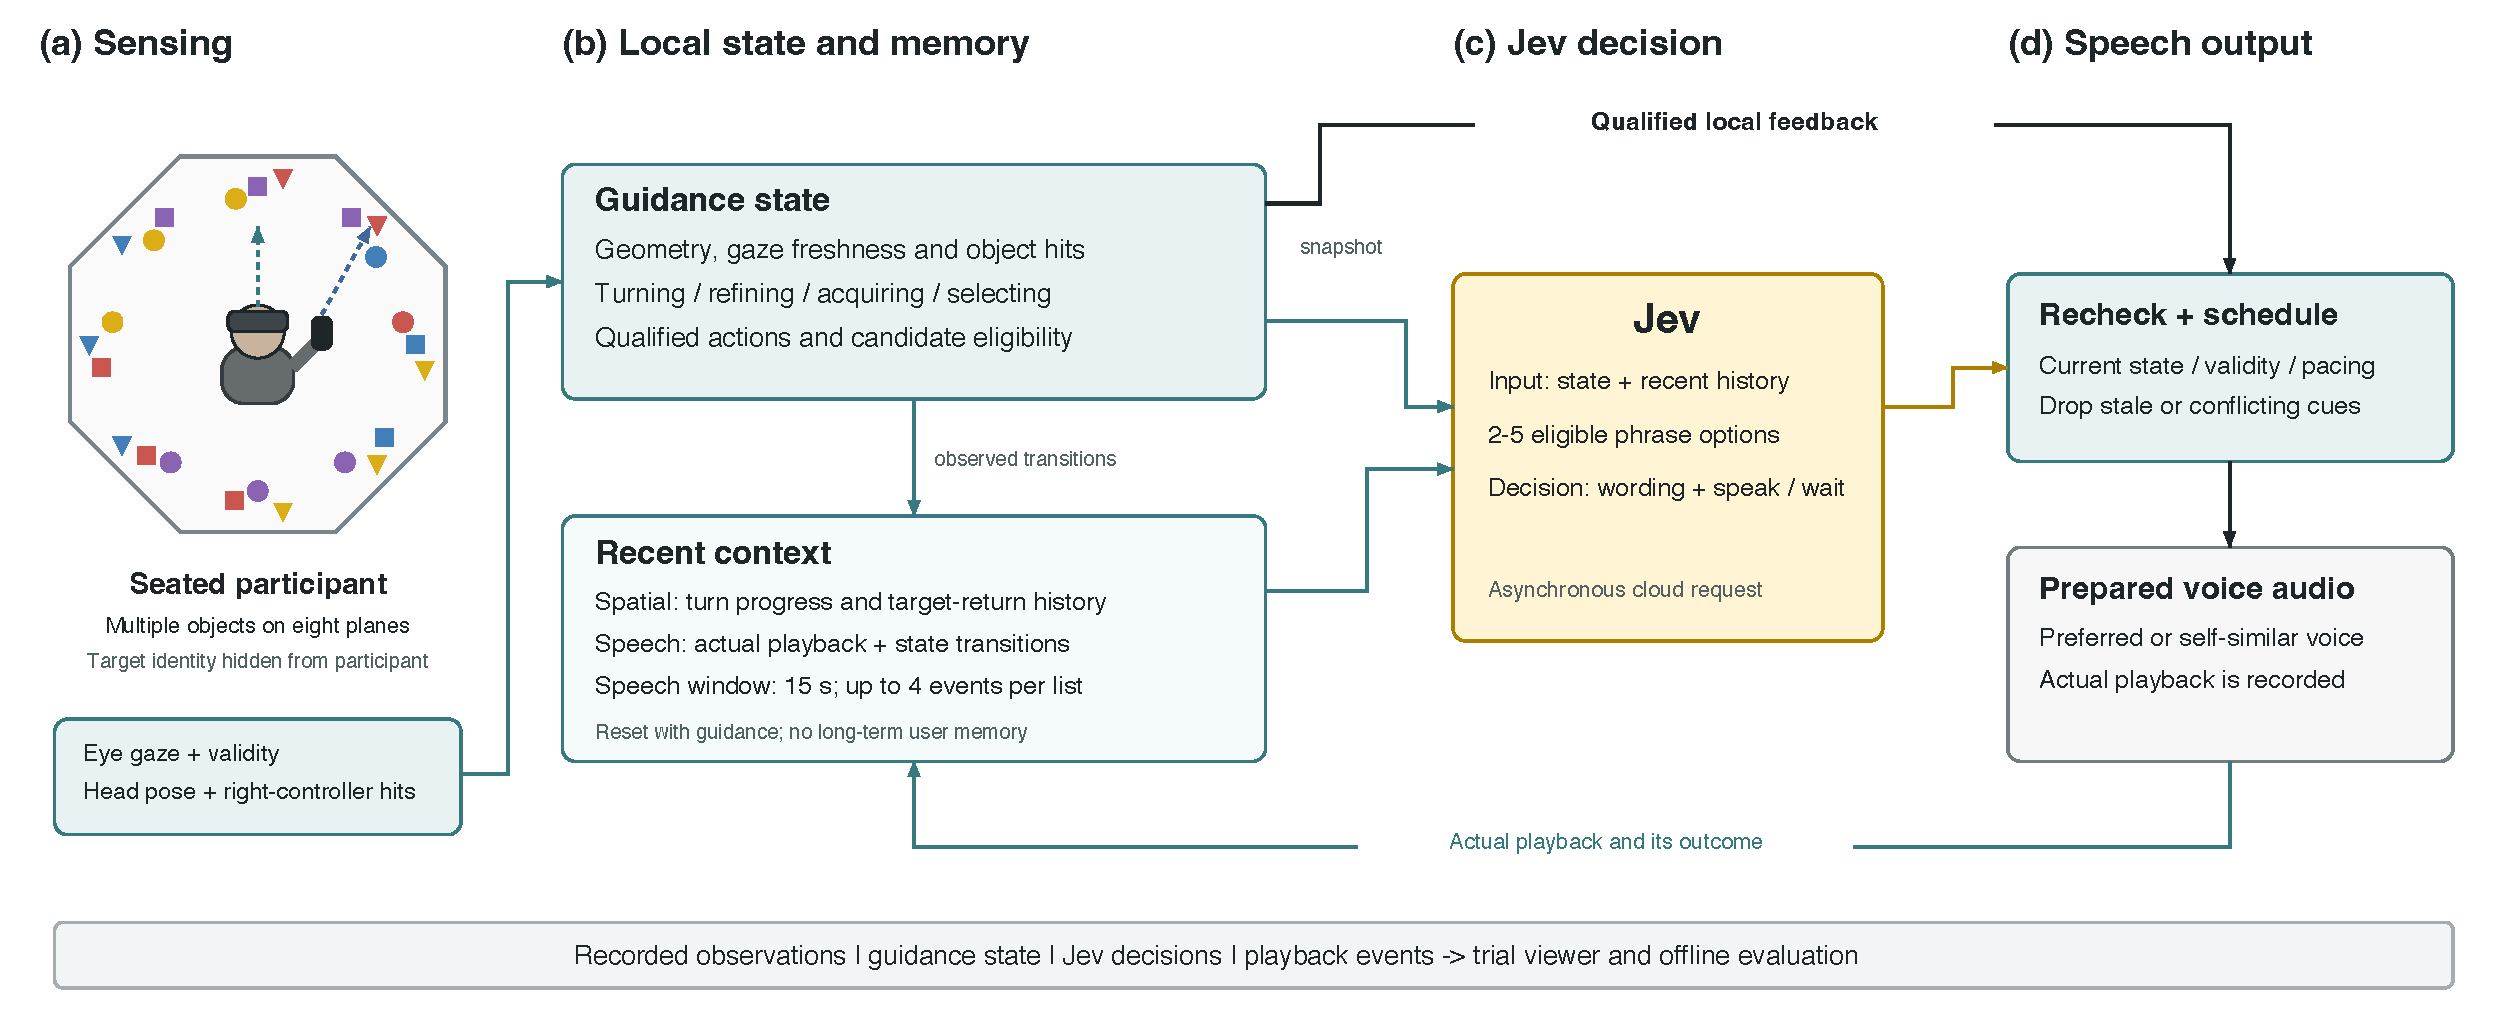
\includegraphics[width=\linewidth,alt={Gaze and controller sensing feed local state and memory, constrained decision-model choices, a fresh playback check, and actual speech feedback.}]{figures/voice-guidance-memory-architecture.pdf}}{\fbox{\parbox{0.94\linewidth}{Gaze and controller observations $\rightarrow$ local state and bounded context $\rightarrow$ eligible choices for the decision model $\rightarrow$ current-state recheck $\rightarrow$ prepared voice playback. Qualified local feedback also enters the recheck stage.}}}
\caption[Guidance architecture and playback control]{System architecture. (a) Gaze, head, and controller data are sensed. (b) A local state machine and short-term memory determine which guidance actions are valid. (c) The MiniLM decision model chooses the strategy and wording from eligible options. (d) The scheduler revalidates each cue against the current state before playback. Actual playback feeds back into memory. The scene inset is schematic and does not reflect stimulus count or any participant-visible target cue.}
\label{fig:architecture}
\end{figure}

Figure~\ref{fig:jev-final-gate} shows the final playback gate. The model's decision is based on an earlier snapshot, so it is treated as advice. A decision to speak results in playback only if the cue passes current-state checks. Provider-selected phrases and qualified local feedback both pass these checks before the prepared clip starts. Readiness and pacing are checked during scheduling, and the queued relevance callback is evaluated again immediately before audio playback. The same local gate applies to every strategy the model can choose.

\begin{figure}[p]
\centering
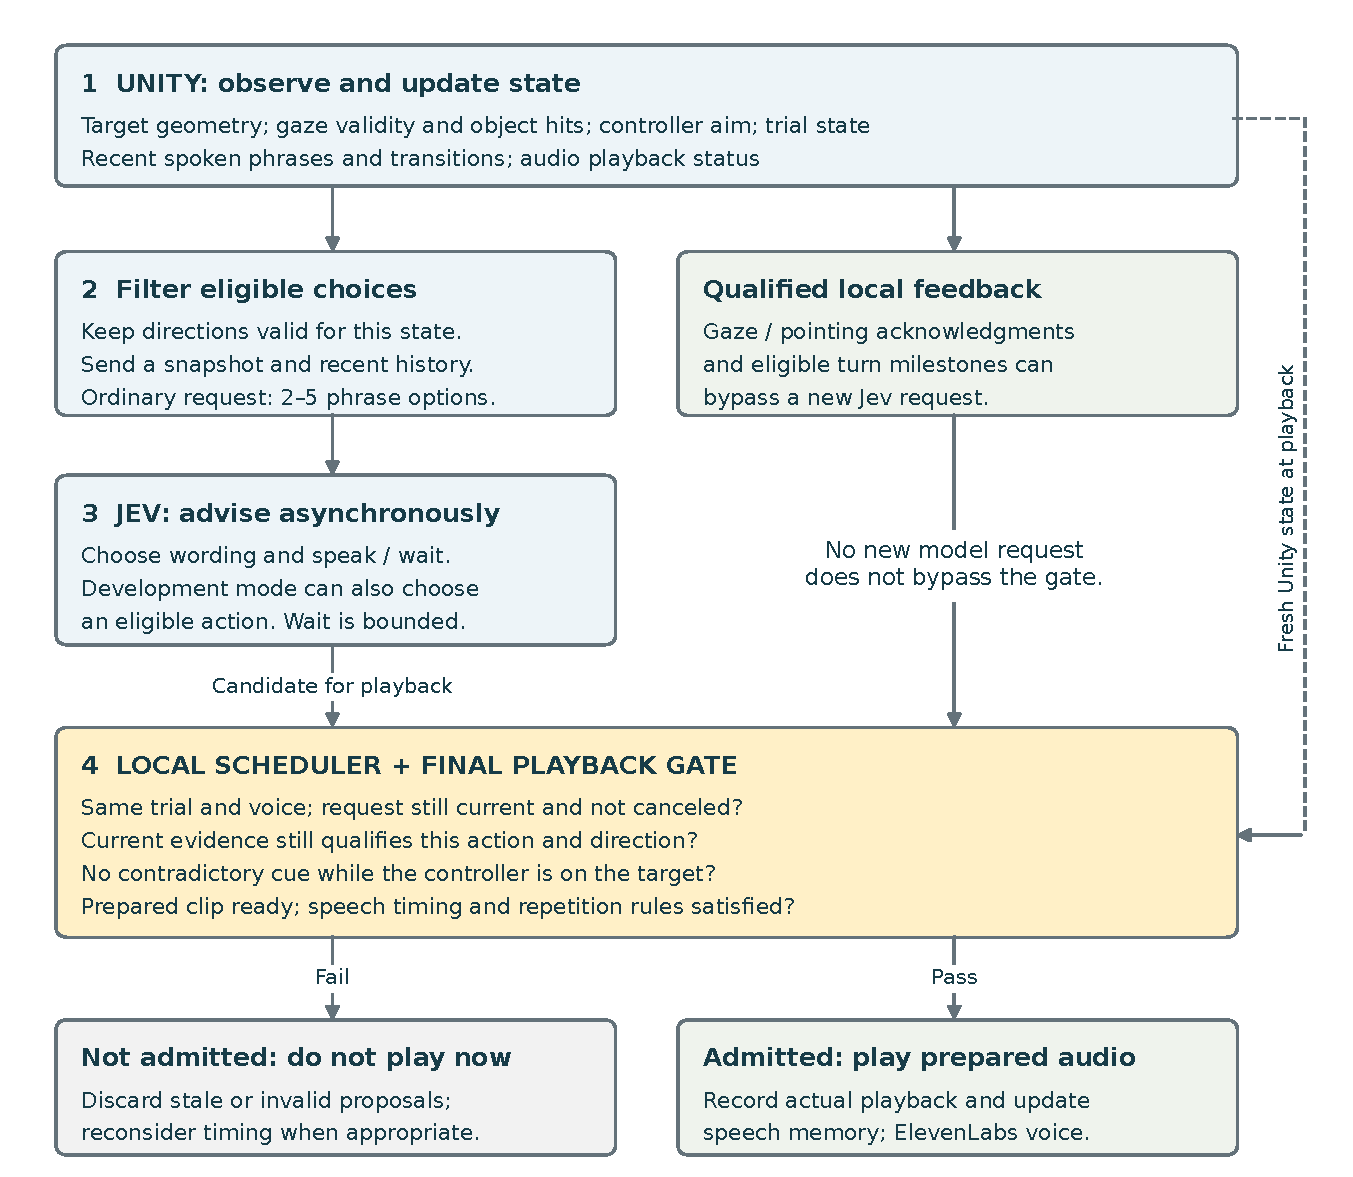
\includegraphics[width=\linewidth,alt={Unity observes current target, gaze, controller, trial and speech state, then filters eligible phrases for the decision model, which chooses the strategy and wording, including whether to speak or wait. Qualified local acknowledgments may bypass a new model request. Both routes enter a final local gate with fresh state, cancellation, qualification, controller conflict, clip readiness, pacing and repetition checks. A failed check prevents immediate playback; an admitted clip plays and updates recorded speech memory.}]{figures/jev-final-playback-gate.pdf}
\caption[Model decisions and the final playback gate]{Decision-model choices and the final local playback gate. The dashed input indicates that the gate evaluates fresh Unity state, not only the snapshot originally sent to the provider. Box 4 groups scheduling checks with the final relevance check immediately before playback. Qualified local feedback bypasses a new model request but retains this boundary. Waiting is bounded by local policy; timeout and deferral fallbacks also pass through the gate. This schematic summarizes ordinary guidance and local feedback rather than every interruption, opening, or success-feedback path. It describes control flow, not measured response latency.}
\label{fig:jev-final-gate}
\end{figure}

\subsubsection{Delivery Quality as an Experimental Requirement}
Both voice conditions use the same versioned guidance mechanism, although delivered sequences depend on participant behavior and clips may differ acoustically. Voice identity, library metadata, playback onset, and delivery faults are therefore recorded so that each can be traced to its condition.

This record matters because a delayed or confusing cue could alter search performance or a participant's judgment of the voice and then be mistaken for an effect of voice condition. Appendix~\ref{app:scenarios} defines guidance sequence tests and an evaluation rubric for checking the implementation.

\subsection{Trial Review Interface}
\label{sec:trial-review}
Figure~\ref{fig:trial-review-synthetic-demo} shows the standalone Trial Review application with its bundled synthetic demonstration. The scene and inspector share a timeline with speech, gaze, events, and decision tracks. The application can also receive headset records for live review. Transfer and receipt times are kept separate from source event times, so late arrival in the viewer does not indicate delayed guidance on the headset. The capture illustrates the interface, not a participant recording or performance result, and the demonstration explicitly marks missing state history and reconstructed highlights.

\begin{figure}[htbp]
\centering
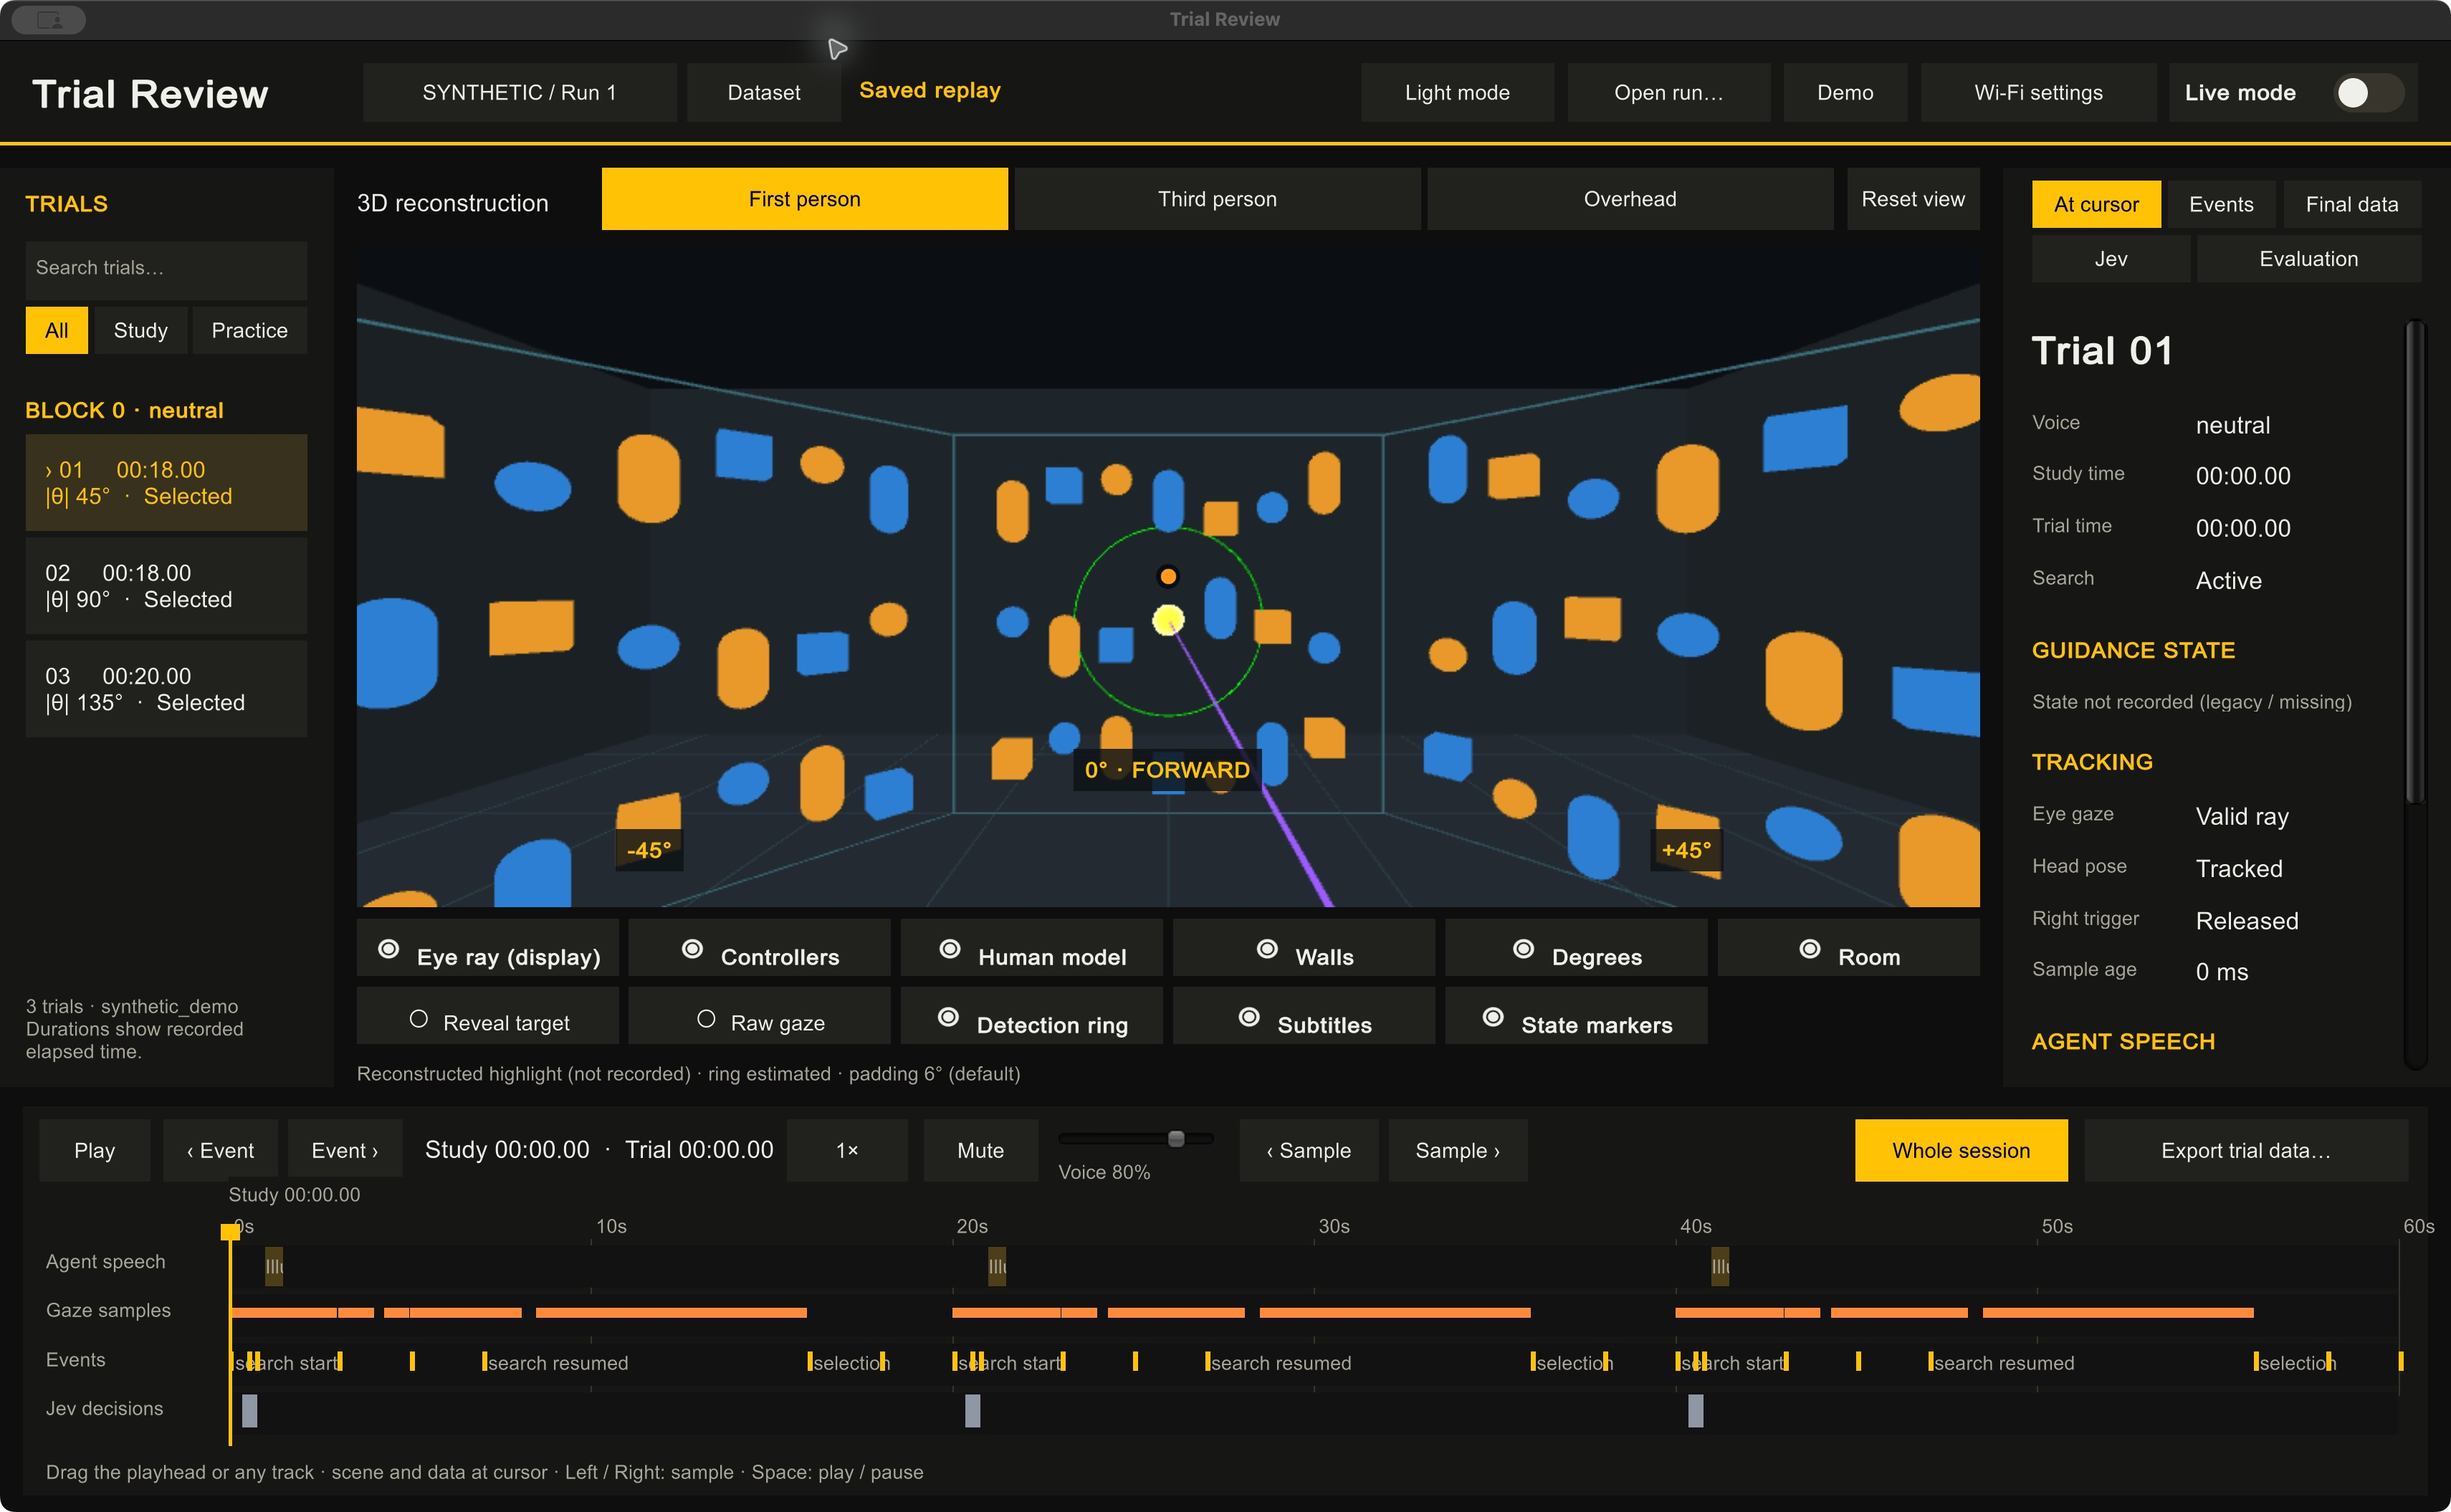
\includegraphics[width=\linewidth,alt={Trial Review application showing its explicitly synthetic three-trial demonstration, reconstructed scene, evidence inspector, and synchronized timeline.}]{figures/trial-review-synthetic-demo.png}
\caption[Trial Review interface with synthetic demonstration]{Application screenshot of the bundled SYNTHETIC / Run 1 demonstration. The central reconstruction, right-hand inspector, and timeline provide synchronized review. Missing state, estimated rings, and reconstructed highlights are labeled by the application. This is a visualization example, not headset video or empirical study data.}
\label{fig:trial-review-synthetic-demo}
\end{figure}



